% Options for packages loaded elsewhere
\PassOptionsToPackage{unicode}{hyperref}
\PassOptionsToPackage{hyphens}{url}
%
\documentclass[
]{article}
\usepackage{amsmath,amssymb}
\usepackage{iftex}
\ifPDFTeX
  \usepackage[T1]{fontenc}
  \usepackage[utf8]{inputenc}
  \usepackage{textcomp} % provide euro and other symbols
\else % if luatex or xetex
  \usepackage{unicode-math} % this also loads fontspec
  \defaultfontfeatures{Scale=MatchLowercase}
  \defaultfontfeatures[\rmfamily]{Ligatures=TeX,Scale=1}
\fi
\usepackage{lmodern}
\ifPDFTeX\else
  % xetex/luatex font selection
\fi
% Use upquote if available, for straight quotes in verbatim environments
\IfFileExists{upquote.sty}{\usepackage{upquote}}{}
\IfFileExists{microtype.sty}{% use microtype if available
  \usepackage[]{microtype}
  \UseMicrotypeSet[protrusion]{basicmath} % disable protrusion for tt fonts
}{}
\makeatletter
\@ifundefined{KOMAClassName}{% if non-KOMA class
  \IfFileExists{parskip.sty}{%
    \usepackage{parskip}
  }{% else
    \setlength{\parindent}{0pt}
    \setlength{\parskip}{6pt plus 2pt minus 1pt}}
}{% if KOMA class
  \KOMAoptions{parskip=half}}
\makeatother
\usepackage{xcolor}
\usepackage[margin=1in]{geometry}
\usepackage{graphicx}
\makeatletter
\def\maxwidth{\ifdim\Gin@nat@width>\linewidth\linewidth\else\Gin@nat@width\fi}
\def\maxheight{\ifdim\Gin@nat@height>\textheight\textheight\else\Gin@nat@height\fi}
\makeatother
% Scale images if necessary, so that they will not overflow the page
% margins by default, and it is still possible to overwrite the defaults
% using explicit options in \includegraphics[width, height, ...]{}
\setkeys{Gin}{width=\maxwidth,height=\maxheight,keepaspectratio}
% Set default figure placement to htbp
\makeatletter
\def\fps@figure{htbp}
\makeatother
\setlength{\emergencystretch}{3em} % prevent overfull lines
\providecommand{\tightlist}{%
  \setlength{\itemsep}{0pt}\setlength{\parskip}{0pt}}
\setcounter{secnumdepth}{-\maxdimen} % remove section numbering
\usepackage{float}
\ifLuaTeX
  \usepackage{selnolig}  % disable illegal ligatures
\fi
\IfFileExists{bookmark.sty}{\usepackage{bookmark}}{\usepackage{hyperref}}
\IfFileExists{xurl.sty}{\usepackage{xurl}}{} % add URL line breaks if available
\urlstyle{same}
\hypersetup{
  pdftitle={Environmental Noise and Ross-Macdonald Transmission Models},
  pdfauthor={Karin Ebey, John Vinson and Kyle Dahlin},
  hidelinks,
  pdfcreator={LaTeX via pandoc}}

\title{Environmental Noise and Ross-Macdonald Transmission Models}
\author{Karin Ebey, John Vinson and Kyle Dahlin}
\date{2023-07-10}

\begin{document}
\maketitle

\hypertarget{outbreak-probability}{%
\section{Outbreak probability}\label{outbreak-probability}}

\hypertarget{number-of-cases}{%
\section{Number of cases}\label{number-of-cases}}

\hypertarget{time-to-outbreak-extinction}{%
\section{Time to outbreak
extinction}\label{time-to-outbreak-extinction}}

\#Results from Julia

\textbackslash begin\{figure\}{[}H{]}

\{\centering 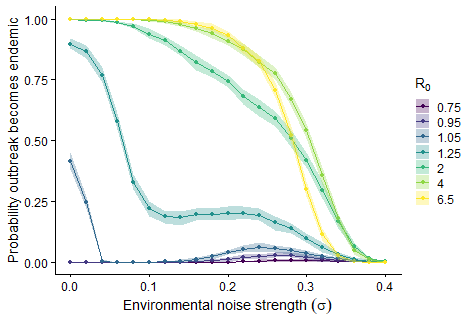
\includegraphics[width=1\linewidth,]{C:/Users/kydah/OneDrive/Documents/GitHub/NoisyMBDs/doc/poster-figures_files/figure-latex/prob_end-1}

\}

\textbackslash caption\{\label{fig:SDEprob_end} Probability of the
disease becoming endemic by sigma and R0 based on 1000 runs of 100
iterations. Overall, increasing environmental noise strength cases the
probability that the disease becomes endemic to decrease. For smaller R0
values (i.e.~\textless1.25), there is a slight increase in endemic
disease probability at high environmental noise levels. Above
environmental noise strength of 0.4 (where there is up to 40\% variation
in parameter values), the probability of endemic disease goes to zero.
There is a greater probability of the disease going endemic at higher
values of R0.\}\label{fig:prob_end} \textbackslash end\{figure\}

\begin{figure}[H]

{\centering 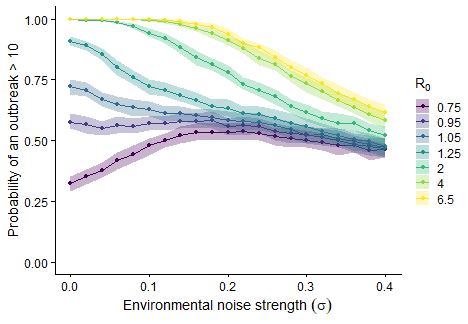
\includegraphics[width=1\linewidth,]{C:/Users/kydah/OneDrive/Documents/GitHub/NoisyMBDs/doc/poster-figures_files/figure-latex/prob_out10-1} 

}

\caption{\label{fig:SDEprob_out10} Probability of an outbreak (defined as 10 host cases at one time point) occuring by sigma and R0 based on 1000 runs of 100 iterations. For R0 values greater than 1, as environmental noise strength increases the probability of an outbreak decreases. For R0 values less than 1, as environmental noise strength increases, the probability of an outbreak increases until sigma=~0.2 and then decreases. There is a greater probability of an outbreak at higher values of R0.}\label{fig:prob_out10}
\end{figure}
\begin{figure}[H]

{\centering 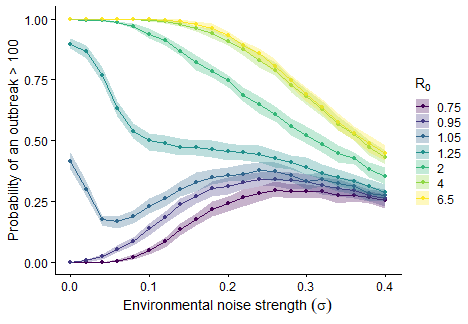
\includegraphics[width=1\linewidth,]{C:/Users/kydah/OneDrive/Documents/GitHub/NoisyMBDs/doc/poster-figures_files/figure-latex/prob_out100-1} 

}

\caption{\label{fig:SDEprob_out100} Probability of an outbreak (defined as 100 host cases at one time point) occuring by sigma and R0 based on 1000 runs of 100 iterations. In general, for R0 values greater than 1, as environmental noise strength increases the probability of an outbreak decreases. For R0 values less than 1, as environmental noise strength increases, the probability of an outbreak increases until sigma=~0.25 and then decreases. R0=1.05 follows both patterns to some degree. There is a greater probability of an outbreak at higher values of R0.}\label{fig:prob_out100}
\end{figure}
\begin{figure}[H]

{\centering 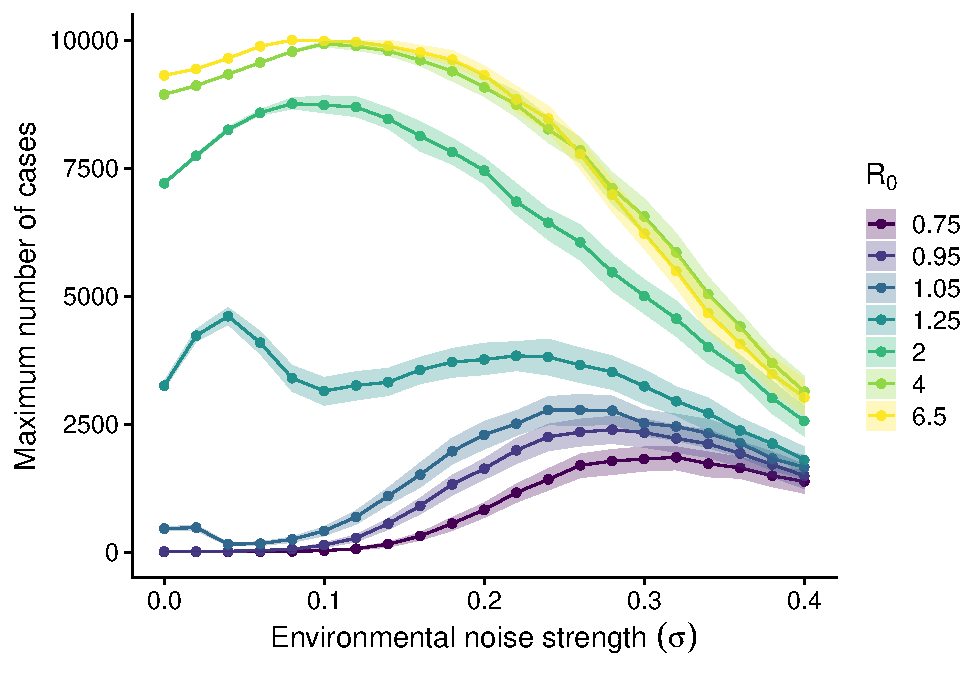
\includegraphics[width=1\linewidth,]{C:/Users/kydah/OneDrive/Documents/GitHub/NoisyMBDs/doc/poster-figures_files/figure-latex/max_cases_all-1} 

}

\caption{\label{fig:SDEmax_cases_all} Maximum number of cases during the simulation by sigma and R0 based on 1000 runs of 100 iterations. For all R0 values, the maximum number of cases increases with environmental noise strength initially and then decreases as environmental noise strength gets too high. For high R0 values, the shift occurs at sigma=~0.15, and for lower R0 values, the shift occurs at sigma=~0.25. R0=1.25 shows intermediate behavior responding at both sigma values. With higher values of R0, more hosts are infected.}\label{fig:max_cases_all}
\end{figure}
\begin{figure}[H]

{\centering 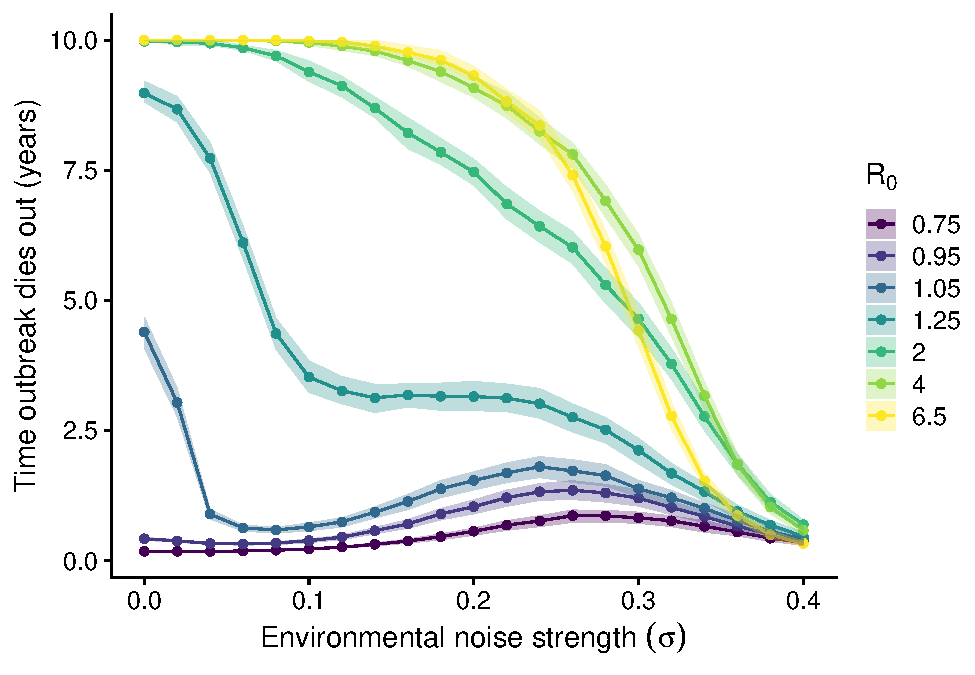
\includegraphics[width=1\linewidth,]{C:/Users/kydah/OneDrive/Documents/GitHub/NoisyMBDs/doc/poster-figures_files/figure-latex/end_time-1} 

}

\caption{\label{fig:SDEend_time} Time that the outbreak dies out (or 10 years-end of simulation) by sigma and R0 based on 1000 runs of 100 iterations. This graph looks quite similar to that of the probability of disease going endemic, because if the disease does not go endemic, the disease goes extinct early on in the simulation.}\label{fig:end_time}
\end{figure}
\begin{figure}[H]

{\centering 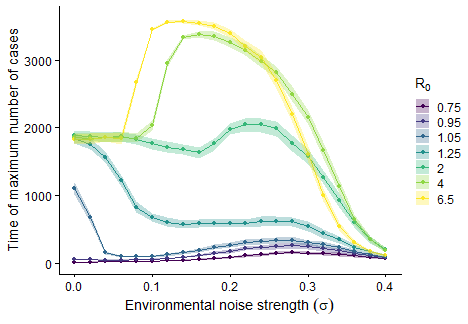
\includegraphics[width=1\linewidth,]{C:/Users/kydah/OneDrive/Documents/GitHub/NoisyMBDs/doc/poster-figures_files/figure-latex/time_max-1} 

}

\caption{\label{fig:SDEtime_max} Time when the maximum number of cases occured during the simulation by sigma and R0 based on 1000 runs of 100 iterations.}\label{fig:time_max}
\end{figure}
\begin{figure}[H]

{\centering 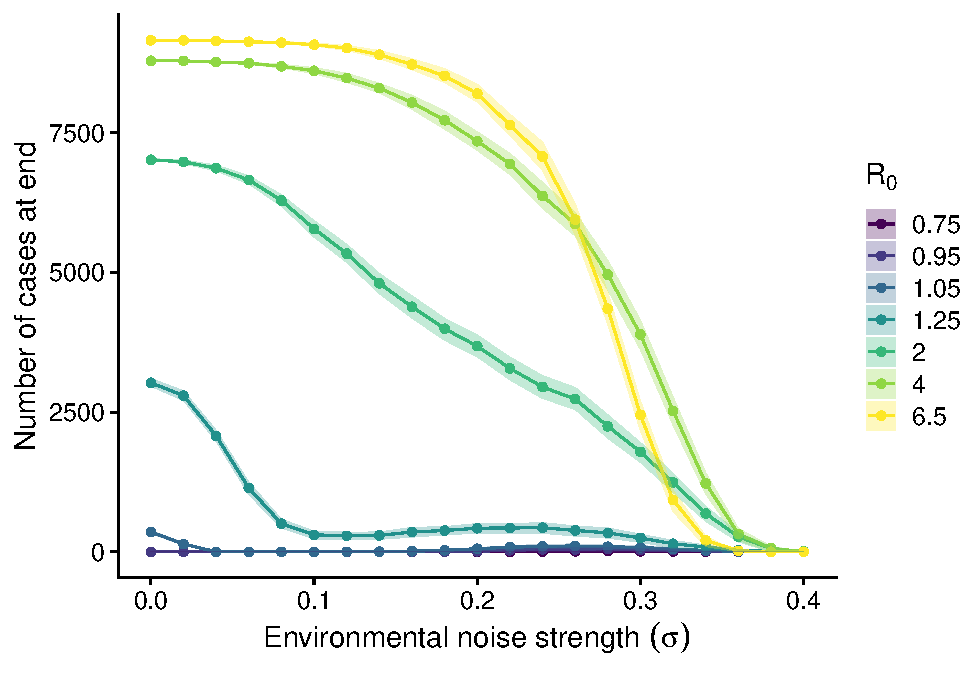
\includegraphics[width=1\linewidth,]{C:/Users/kydah/OneDrive/Documents/GitHub/NoisyMBDs/doc/poster-figures_files/figure-latex/num_cases-1} 

}

\caption{\label{fig:SDEnum_cases} Number of host cases at the end of the simulation by sigma and R0 based on 1000 runs of 100 iterations. This graph looks similar to that of the probability of disease going endemic, because if the disease does not go endemic, then zero hosts are infected at the end. More hosts are infected at higher R0 values.}\label{fig:num_cases}
\end{figure}

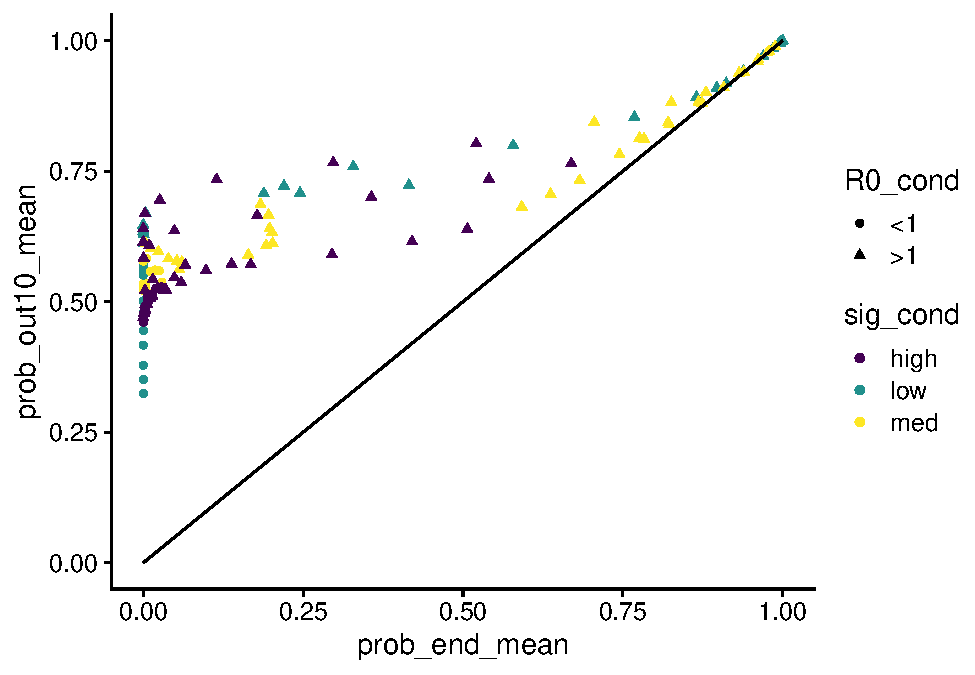
\includegraphics{C:/Users/kydah/OneDrive/Documents/GitHub/NoisyMBDs/doc/poster-figures_files/figure-latex/unnamed-chunk-3-1}

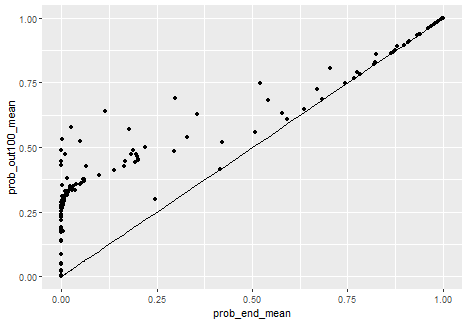
\includegraphics{C:/Users/kydah/OneDrive/Documents/GitHub/NoisyMBDs/doc/poster-figures_files/figure-latex/unnamed-chunk-4-1}

\#Trajectories Plot

\begin{figure}[H]

{\centering 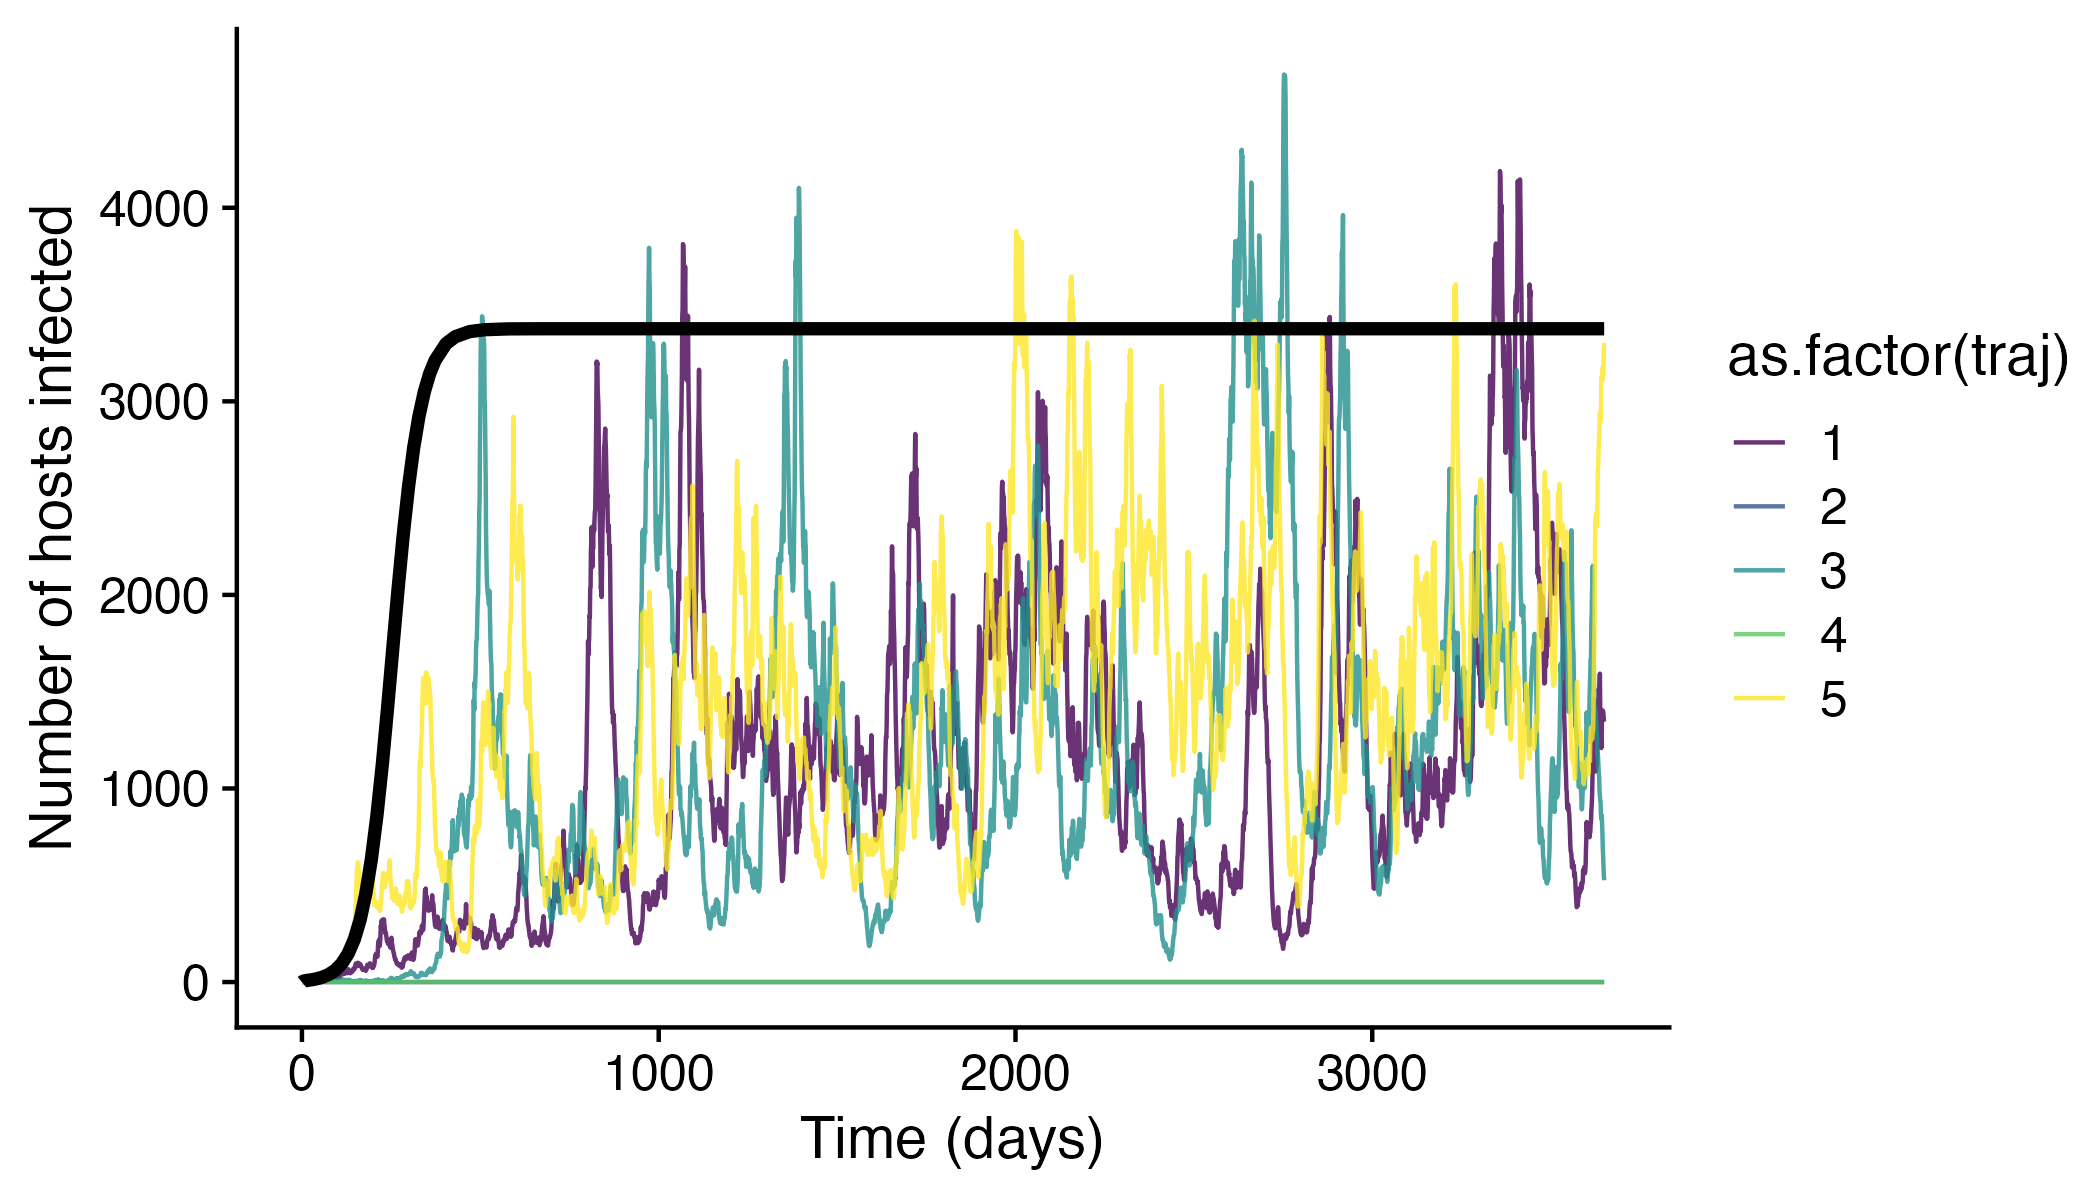
\includegraphics[width=1\linewidth,]{C:/Users/kydah/OneDrive/Documents/GitHub/NoisyMBDs/doc/poster-figures_files/figure-latex/trajectories-1} 

}

\caption{\label{fig:SDEtrajectories} For R0=1.25 and sigma=0.08, the number of hosts infected at each time period in deterministic solution (black line) and 5 stochastic solutions (colored lines) are plotted.}\label{fig:trajectories}
\end{figure}

```

\begin{figure}[H]

{\centering 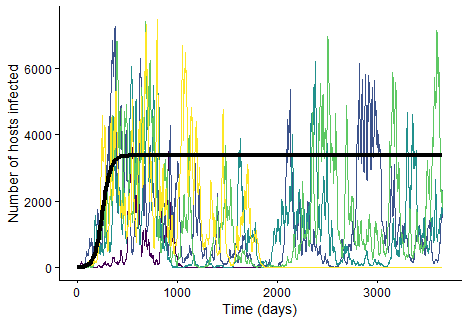
\includegraphics[width=1\linewidth,]{C:/Users/kydah/OneDrive/Documents/GitHub/NoisyMBDs/doc/poster-figures_files/figure-latex/trajectories-2-1} 

}

\caption{\label{fig:SDEtrajectories} For R0=1.25 and sigma=0.08, the number of hosts infected at each time period in deterministic solution (black line) and 5 stochastic solutions (colored lines) are plotted.}\label{fig:trajectories-2}
\end{figure}

\end{document}
